\documentclass[a4paper,12pt]{article}

\usepackage{float}
\usepackage{url}
\usepackage{setspace}
\usepackage[portuguese]{babel}
\setstretch{1.25}
\usepackage{graphicx}
\usepackage{colortbl}
\usepackage{url}
\usepackage[margin=1.1in]{geometry}
\graphicspath{ {./images/} }

% correct bad hyphenation here
\hyphenation{op-tical net-works semi-conduc-tor}


\begin{document}
\title{
	\begin{center}
		
\includegraphics[scale=0.5]{logofct.pdf}
	\end{center}
	Estatística Multivariada \\ \small{Análise Global de Suicídios (1985-2016)}}
\author{João Pedro de Noronha Funenga \\ MAEBD - Nº 61635 \\ j.funenga@campus.fct.unl.pt}


\maketitle
\newpage

\tableofcontents
\newpage

\listoffigures
\listoftables
\newpage


\section{Introdução}
Este projeto no âmbito da unidade curricular de \textit{Estatística Multivariada} terá como objetivo \underline{analisar as taxas mundiais de suicídio} e tirar algumas conclusões práticas a partir dos dados. Existem esterótipos e preconceitos pré-existentes acerca deste tema, como por exemplo, os homens serem o grupo predominante entre as vítimas ou pessoas de idade avançada tenderem a optar por esta saída (muitas das vezes devido a doenças crónicas ou faltas de apoio do estado). Neste trabalho irei testar se de facto os dados corroboram as teorias prévias ou não. Visto existirem países com condições e enquadramentos socioeconómicos muito díspares, julgo que uma boa forma de abordar o problema será \underline{criando grupos (\textit{clusters})} definidos por um conjunto de variáveis e veremos como estes de facto se encontram espacialmente separados e existem diferenças significativas entre estes.


\section{Descrição do \textit{dataset}}
Como falado na introdução, para este trabalho decidi escolher um conjunto de dados relativos aos suicídios entre 1985 e 2016. Para além do número
de suicídios, também existem as colunas relativas ao grupo etário (com os 5 intervalos de 15-24, 25-34, 35-54, 55-74, 75+ anos), ao género, ao país e respetiva população e PIB per capita. Existem outras colunas
adicionais mas que não utilizarei.  

\section{Metodologia}
Para este projeto, utilizarei um dos mais conhecidos algoritmos de clustering, o \textbf{\textit{k-means}}. Este algoritmo funciona agrupando os dados em \textit{k} grupos (sendo \textit{k} um parâmetro que precisamos de passar). Cada um dos grupos será representado pelo seu centróide (ponto médio do cluster). Por sua vez, cada um dos pontos (que correspondem a uma observação do ficheiro \textit{"suicides.csv"}), será atribuído ao cluster cuja \textbf{distância euclidiana ao centróide correspondente é menor}. Para cada iteração do algoritmo, a posição dos centróides vai alterando o que também afeta a que cluster é que os exemplos são alocados. Este algoritmo tem como condição terminal a não alteração da atribuição dos exemplos aos clusters entre iterações consecutivas.
Por vezes, ao aplicarmos este algoritmo, temos como ideia o número de \textit{clusters} finais que queremos. No entanto, este não é o caso. De modo a calcular o número de grupos ideal, irei recorrer a uma técnica falada em aula. Esta técnica é chamada de \textbf{\textit{Silhouette Method}} e funciona da seguinte forma:
\begin{enumerate}
	\item Realizar a análise de clusters considerando um \textbf{intervalo de valores para k} (no meu caso k $\in$ [1,10])
	\item Para cada valor de k, \textbf{calcular a média dos coeficientes de \textit{Silhouette}}
	\item Representar o gráfico que relaciona os \textit{k} testados com a média dos coeficientes \textit{Silhouette} entre todos os clusters.
	\item O valor escolhido para \textit{k} corresponderá ao \textbf{máximo da função} (em que a média dos coeficientes \textit{Silhouette} têm o valor mais alto).
\end{enumerate}
Depois de ter os clusters calculados e as respetivas observações agrupadas, irei analisar cada um deles e verificar se existe algum padrão que seja possível de revelar.

\section{\textit{Overview} Inicial}
Primeiramente, iremos olhar para a evolução da taxa média de suicídios desde 1985 até 2016.

\begin{center} %8 9
	\begin{figure}[H]
		\centering
		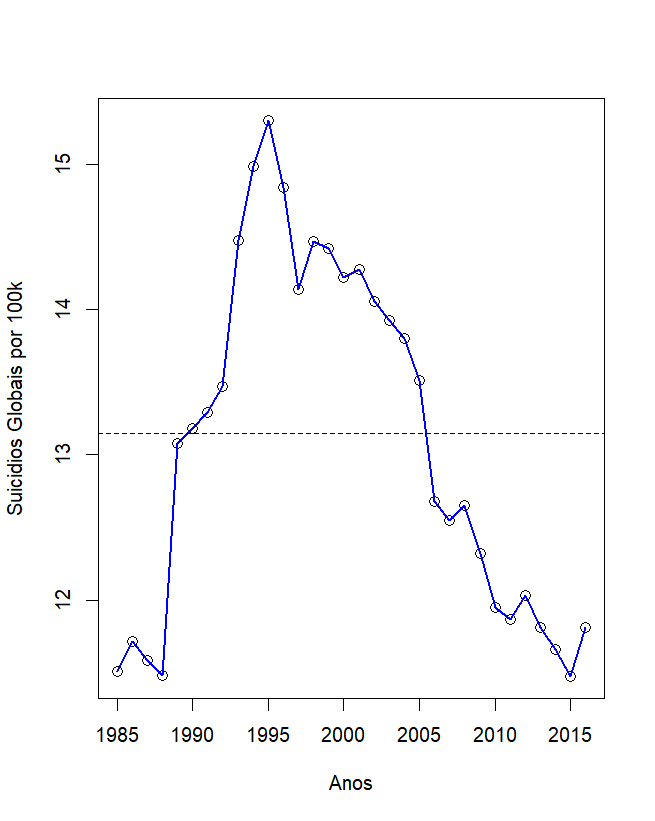
\includegraphics[width=7cm, height=6cm]{taxaMediaSuicidios100k.png}
		\caption{Taxa de suicídio ao longo dos anos}
	\end{figure}
\end{center}
Como podemos observar, esta parece estar a decrescer desde aproximadamente 1995 e, anteriormente a esta data, os números eram bastante mais baixos. Possivelmente,
isto pode ser explicado por nesta altura não haver um registo deste tipo de dados tão minucioso como agora e que uma boa parte dos que aconteciam não eram sequer registados como tal. O decréscimo desde o final do milénio pode estar relacionado com a banalização e massificação de se falar sem preconceitos da saúde mental. Para além disto, no gráfico também representei a \textbf{taxa média de suícidos global} com a linha a traçejado, que se situa nos \textbf{13.15 por 100.000 pessoas}.


\section{Procedimento}
Tendo a metodologia a usar sido explicada em cima, irei agora explicar como procedi. Primeiramente, decidi ajustar o \textit{dataset} de modo a facilitar o uso posterior. Algumas das alterações que realizei foram a alteração de nomes das colunas bem como descartar outras que não fariam sentido serem utilizadas. Um aspeto importante a referir foi a questão de necessitar de \textbf{padronizar os dados}. Ao observar os valores dos atributos que irei analisar e que servirão para a constituição dos clusters, é possível perceber que estão em escalas e unidades completamente diferentes o que me leva a ter de os \textit{standardizar} usando a função \textit{scale}. Inicialmente, por uma questão experimental, tentei perceber qual seria o resultado de não os escalar e, utilizando o número de grupos dado pelo método da \textit{silhouette} (neste caso seriam 2 grupos), os dados apresentavam-se agrupados de uma forma que não fazia qualquer sentido, sendo assim outro fator que me levou a realizar este pré-processamento.

Como enunciado, o algoritmo \textit{k-means} tem como parâmetro o \textbf{número de \textit{clusters}} e este foi obtido da forma explicada na metodologia. Dando uso a funções \textit{built-in} do R, fiz a representação gráfica da relação entre o número de grupos e o valor médio do coeficiente de \textit{Silhouette}. 


\begin{center} %8 9
	\begin{figure}[H]
		\centering
		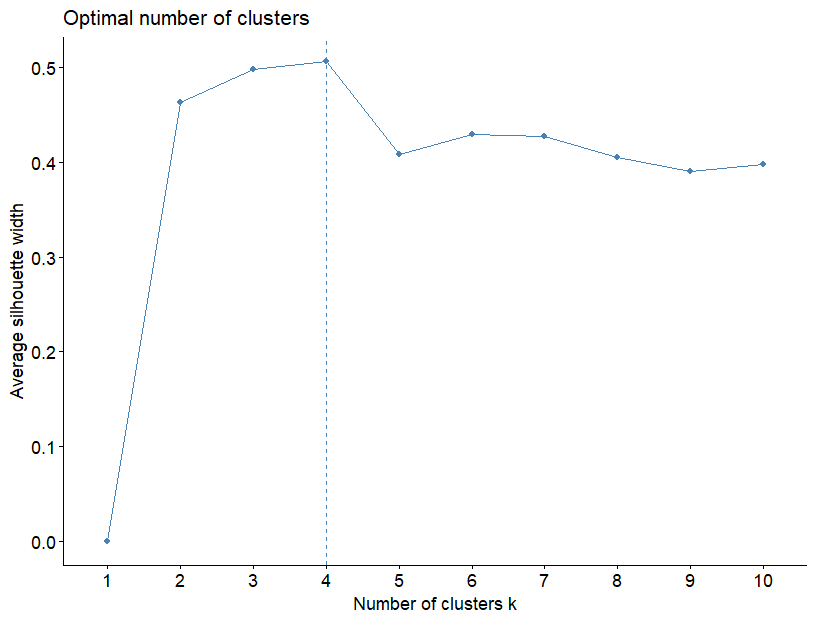
\includegraphics[width=10cm, height=7cm]{clusteringSilhouetteComStandardizacao.png}
		\caption{Coeficiente \textit{Silhouette} vs nº de clusters}
		\label{fig:silhouette}
	\end{figure}
\end{center}


Como podemos ver pelo gráfico, o número ideal de \textit{clusters} a utilizar é de 4, o que, comparado aos 2 dados utilizando os dados não \textit{standardizados} faz muito mais sentido.
Agora que tenho o valor para o parâmetro \textit{k}, posso então utilizar a função do R para realizar o algoritmo em si. Esta função tem como \textbf{parâmetros} os \textbf{dados correspondentes aos atributos} a serem utilizados, o \textbf{número de \textit{clusters}} e o \textbf{número de inícios aleatórios} que serão feitos. 


Para o \underline{primeiro argumento}, os atributos que decidi utilizar para a representação dos clusters foram a \textbf{população do país}, o \textbf{número de suicídios por 100.000} pessoas bem como o \textbf{\textit{PIB per capita} do país}. Julgo que a combinação destas três \textit{features} será representativa para separar as observações nos vários grupos, isto porque são fatores que muitas das vezes estão relacionados entre si, têm uma fácil interpretação e diferem bastante globalmente.


Para o \underline{segundo argumento}, como vimos, o número de \textit{clusters} a serem gerados é de 4, o correspondente ao máximo da imagem \ref{fig:silhouette}.


Relativamente ao último e \underline{terceiro argumento}, este representa o número de inícios aleatórios que o algoritmo fará. Basicamente, o \textit{k-means} começa por atribuir aleatoriamente a posição dos centróides que utilizará mas, como é natural, existem combinações de posições melhores que as outras. Por exemplo, caso os 4 centróides fossem todos colocados muito próximos uns dos outros, isto levaria a que os grupos gerados não fizessem grande sentido em termos de interpretação e por isto, com este argumento serão feitos \textit{n} inícios e será escolhido o que melhor separar os dados (o que tiver uma variância intra-cluster baixa), para este parâmetro decidi utilizar um valor de 10 (cf. \cite{nstart}).

Analisaremos então o gráfico que demonstra os 4 agrupamentos dos dados.

\begin{center} %8 9
	\begin{figure}[H]
		\centering
		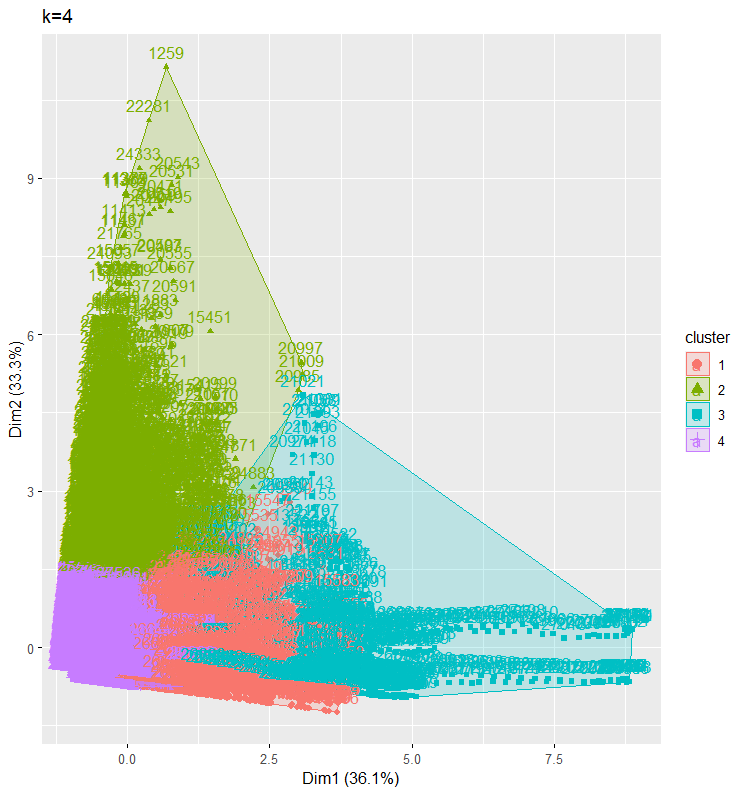
\includegraphics[width=10cm, height=7cm]{clusters4.png}
		\caption{Clusters Gerados}
		\label{fig:clusters}
	\end{figure}
\end{center}


Analisando o gráfico percebemos que os 4 grupos formados têm formas muito diferentes bem como o número de elementos que os constituem.

\begin{table}[H]
	\centering
	\caption{Número de elementos dos clusters}
	\begin{tabular}{|c|c|c|c|} 
		\hline
		\rowcolor[rgb]{0.706,0.922,0.996} Cluster 1 & Cluster 2 & Cluster 3 & Cluster 4  \\ 
		\hline
		4448                                        & 2321      & 1429      & 19622      \\
		\hline
	\end{tabular}
\end{table}



A sobreposição que se verifica no gráfico está relacionada com o número de atributos selecionados (que correspondem à dimensão do espaço). Por ter escolhido 3 atributos e estar a fazer a representação num espaço bi-dimensional, existem pontos que se encontram sobrepostos.

\section{Análise dos Clusters}

Com os 4 clusters que obtive, irei analisar cada um e verificar o que, aproximadamente, cada um deles pode representar.

\begin{table}[H]
	\centering
	\caption{Valores médios}
	\label{table:medios}
	\begin{tabular}{|c|c|c|c|} 
		\hline
		\rowcolor[rgb]{0.706,0.922,0.996} \multicolumn{1}{|l|}{} & \textbf{ População } & \textbf{~ ~Suicídios/100k~~ } & \textbf{PIB \textit{per capita} (\$)}  \\ 
		\hline
		{\cellcolor[rgb]{0.706,0.922,0.996}}\textbf{Cluster 1}   & 1384540.5            & 11.0                          & 50607.8                           \\ 
		\hline
		{\cellcolor[rgb]{0.706,0.922,0.996}}\textbf{Cluster 2}   & 1130833.3            & 62.3                          & 12041.4                           \\ 
		\hline
		{\cellcolor[rgb]{0.706,0.922,0.996}}\textbf{Cluster 3}   & 15487347.9           & 12.0                          & 21008.5                           \\ 
		\hline
		{\cellcolor[rgb]{0.706,0.922,0.996}}\textbf{Cluster 4}   & 1040038.6            & 7.4                           & 9486.9                            \\
		\hline
	\end{tabular}
\end{table}


\subsection{Cluster 1}
Analisando os valores médios para o primeiro \textit{cluster}, percebemos que este tem um \textbf{PIB} de aproximadamente 50k\$, sendo assim o \textbf{mais alto dos 4}. Olhando agora para os suicidios por 100k pessoas, percebemos que este tem um valor de apenas \textbf{11} por cada cem mil pessoas, sendo assim o \textbf{segundo com os números mais baixos}. Relativamente à população média, os países que o constituem têm um valor aproximadamente de pouco menos de 1 milhão e meio de pessoas, o que é um número bastante baixo. Isto aparenta transmitir a mensagem de que \textbf{quem vive em países não muito grandes com uma boa qualidade económica, não tende a optar por esta saída.}
Veremos agora, das observações, quais são os 5 países que mais aparecem neste cluster.


\begin{table}[H]
	\centering
	\caption{Cluster 1 - Países Frequentes}
	\begin{tabular}{|c|c|} 
		\hline
		\rowcolor[rgb]{0.678,1,0.851} País & Nº Ocorrências  \\ 
		\hline
		Luxemburgo                         & 300             \\ 
		\hline
		Noruega                            & 297             \\ 
		\hline
		Dinamarca                          & 252             \\ 
		\hline
		Suiça                              & 238             \\ 
		\hline
		Islândia                           & 226             \\
		\hline
	\end{tabular}
\end{table}
Ao analisarmos a tabela supradita, percebemos que, para os países com mais ocorrências no cluster, \textbf{todos eles são europeus}. Isto vai ao encontro de o que podemos pensar. Países europeus têm um \textit{PIB per capita} elevado e não apresentam um número muito elevado de suicídios.
Para além dos países que o constituem, veremos agora em que faixa etária é que há mais prevalência de suicídios.

\begin{table}[H]
	\centering
	\caption{Cluster 1 - Frequências nas várias faixas etárias}
	\begin{tabular}{|c|c|} 
		\hline
		\rowcolor[rgb]{0.678,1,0.851} Faixa Etária & Nº Ocorrências  \\ 
		\hline
		25-34        & 793             \\ 
		\hline
		15-24        & 785             \\ 
		\hline
		5-14         & 755             \\ 
		\hline
		55-74        & 734             \\ 
		\hline
		35-54        & 691             \\ 
		\hline
		75+          & 690             \\
		\hline
	\end{tabular}
\end{table}

Pela tabela acima, percebemos que o número de suicídios é bastante \textbf{homogéneo ao longo das várias faixas etárias.} No entanto, tem uma maior prevalência nas gerações \textbf{mais jovens} que nas com mais idade.
Por último, veremos a proporção de homens para mulheres.
\begin{table}[H]
	\centering
	\caption{Cluster 1 - Frequências nos géneros}
	\begin{tabular}{|c|c|} 
		\hline
		\rowcolor[rgb]{0.2,0.7,0.6} Género   & Nº Ocorrências  \\ 
		\hline
		Mulheres & 2241            \\ 
		\hline
		Homens   & 2207            \\
		\hline
	\end{tabular}
\end{table}

Neste caso podemos observar que o número de suicídios em \textbf{homens e mulheres foi muito semelhante} e não aparenta representar o esterótipo que existe.

Relativamente ao valor de variabilidade intra-cluster, este apresenta um de 7158.1. Por este valor por si só não ter grande significado, será depois comparado quando chegar ao último \textit{cluster}.

\subsection{Cluster 2}
Veremos agora o que acontece no segundo \textit{cluster}. A primeira coisa que se destaca é o \textbf{elevado número de suicídios} por cem mil habitantes. Para além disto, o \textbf{\textit{PIB}} é também bastante \textbf{inferior ao primeiro}, cerca de 5 vezes menos. Relativamente ao número médio da população, este é bastante semelhante ao primeiro. Este cluster aparenta representar o \textbf{estereótipo de que países com menos capital} sofrem de uma \textbf{maior taxa de suicídio} entre os seus habitantes. Com isto, analisaremos agora os 5 primeiros países.

\begin{table}[H]
	\centering
	\caption{Cluster 2 - Países Frequentes}
	\begin{tabular}{|c|c|} 
		\hline
		\rowcolor[rgb]{0.678,1,0.851} País & Nº Ocorrências  \\ 
		\hline
		Cazaquistão                        & 121             \\ 
		\hline
		Ucrânia                            & 111             \\ 
		\hline
		Lituânia                           & 107             \\ 
		\hline
		Hungria                            & 98              \\ 
		\hline
		Bielorrússia                       & 90              \\
		\hline
	\end{tabular}
\end{table}

No primeiro cluster tivémos países maioritariamente da europa central e ocidental que, por norma, têm melhor reputação em diversos índices de felicidade (cf. \cite{indicefelicidade}).
Agora, ao vermos a tabela acima percebemos que todos os países que constituem este cluster ou são da \textbf{europa de leste ou asiáticos}, como é o caso do Cazaquistão. Esta análise vai de encontro com as ideias pré-formuladas que existem acerca destas zonas. Pela \textbf{qualidade de vida ser menor}, ressalvando ser uma generalização, aliada aos \textbf{baixos vencimentos}, o \textbf{número de suicídios} demonstra ser bastante mais \textbf{alto} que nos outros grupos.
De seguida vamos ver quais são os grupos etários que mais aparecem neste \textit{cluster}.


\begin{table}[H]
	\centering
	\caption{Cluster 2 - Frequências nas várias faixas etárias}
	\begin{tabular}{|c|c|} 
		\hline
		\rowcolor[rgb]{0.678,1,0.851} Faixa Etária & Nº Ocorrências  \\ 
		\hline
		75+                                        & 1003            \\ 
		\hline
		55-74                                      & 527             \\ 
		\hline
		35-54                                      & 400             \\ 
		\hline
		25-34                                      & 276             \\ 
		\hline
		15-24                                      & 115             \\ 
		\hline
		5-14                                       & 0               \\
		\hline
	\end{tabular}
\end{table}

Ao contrário do que acontece no primeiro cluster relativamente à taxa de suicídios ser parecida nas várias faixas etárias, neste caso conseguimos claramente perceber que o número é aproximadamente o \textbf{dobro para pessoas no final de vida}. Este seria o pressuposto que muitos de nós faríamos, por haver uma panóplia de fatores que podem fazer alguém mais velho não querer continuar, sendo o caso mais comúm o da presença de doenças crónicas ou mesmo o da falta de apoio do estado no que toca a reformas (cf. \cite{suicidioidosos}). 
Para as camadas mais jovens, felizmente o número não é tão elevado.
Por último, veremos a proporção de homens para mulheres.
\begin{table}[H]
	\centering
	\caption{Cluster 2 - Frequências nos géneros}
	\begin{tabular}{|c|c|} 
		\hline
		\rowcolor[rgb]{0.2,0.7,0.6} Género   & Nº Ocorrências  \\ 
		\hline
		Homens & 2222            \\ 
		\hline
		Mulheres   & 99            \\
		\hline
	\end{tabular}
\end{table}

Neste cluster já podemos ver claras diferenças entre os homens e as mulheres, sendo o dos \textbf{homens muito mais elevado}, por aproximadamente 22 vezes.

Relativamente ao valor de variabilidade intra-cluster, este apresenta um valor de 5667.3. 

\subsection{Cluster 3}

Para o terceiro cluster, percebemos que a \textbf{população} média é \textbf{bastante mais elevada} que nos outros. Relativamente ao número de suicídios, este é o segundo mais alto mas longe do que acontece no segundo \textit{cluster}. O PIB deste grupo é cerca do dobro do segundo \textit{cluster}. Veremos quais são os países que lideram neste.


\begin{table}[H]
	\centering
	\caption{Cluster 3 - Países Frequentes}
	\begin{tabular}{|c|c|} 
		\hline
		\rowcolor[rgb]{0.678,1,0.851} País & Nº Ocorrências  \\ 
		\hline
		EUA~                               & 338             \\ 
		\hline
		Brasil                             & 275             \\ 
		\hline
		Rússia                             & 192             \\ 
		\hline
		México                             & 186             \\ 
		\hline
		Japão                              & 182             \\
		\hline
	\end{tabular}
\end{table}

Analisando a tabela, percebemos que os \textbf{países} que constituem este cluster são \textbf{bastante diferentes} em termos culturais e económicos, embora todos sejam bastante grandes e com uma elevada população, podendo ter sido este o fator prevalente em agrupá-los. O outro possivelmente foi o PIB, visto alguns destes serem as maiores potências mundiais. Esta divergência nos países que o constituem pode estar relacionada com, na representação gráfica \ref{fig:clusters} vermos que o cluster 3 se \textbf{alonga bastante para o lado direito do gráfico}.
Observemos agora o que acontece com as faixas etárias.


\begin{table}[H]
	\centering
	\caption{Cluster 3 - Frequências nas várias faixas etárias}
	\begin{tabular}{|c|c|} 
		\hline
		\rowcolor[rgb]{0.678,1,0.851} Faixa Etária & Nº Ocorrências  \\ 
		\hline
		35-54                                       & 453            \\ 
		\hline
		15-24                                      & 256            \\ 
		\hline
		5-14                                      & 249            \\ 
		\hline
		55-74                                      & 226            \\ 
		\hline
		25-34                                      & 214            \\ 
		\hline
		75+                                        & 31            \\
		\hline
	\end{tabular}
\end{table}

Assim como acontece no primeiro cluster, a taxa de suicídios para todos os \textbf{grupos etários} é bastante \textbf{semelhante excepto para as pessoas no final e meio da vida}.
Por último, veremos a proporção de homens para mulheres.

\begin{table}[H]
	\centering
	\caption{Cluster 3 - Frequências nos géneros}
	\begin{tabular}{|c|c|} 
		\hline
		\rowcolor[rgb]{0.2,0.7,0.6} Género   & Nº Ocorrências  \\ 
		\hline
		Mulheres & 760            \\ 
		\hline
		  Homens & 669            \\
		\hline
	\end{tabular}
\end{table}

Assim como no primeiro, temos que o número de suicídios nas \textbf{mulheres é ligeiramente mais alto}, mas não com a proporção que existia no segundo.

Relativamente ao valor de variabilidade intra-cluster, este apresenta um valor de 6442.6.

\subsection{Cluster 4}

Finalmente, veremos o quarto cluster. Pela tabela dos valores médios \ref{table:medios}, percebemos que os países que constituem este \textit{cluster} têm também um \textbf{número baixo de habitantes} embora o seu \textbf{PIB e taxa de suicídios} sejam os \textbf{mais baixos de todos}. Olharemos agora para os países constituintes.


\begin{table}[H]
	\centering
	\caption{Cluster 4 - Países Frequentes}
	\begin{tabular}{|c|c|} 
		\hline
		\rowcolor[rgb]{0.678,1,0.851} País & Nº Ocorrências  \\ 
		\hline
		Colômbia                           & 372             \\ 
		\hline
		Equador                            & 372             \\ 
		\hline
		Malta                              & 370             \\ 
		\hline
		Maurícia                           & 366             \\ 
		\hline
		Chile                              & 361             \\
		\hline
	\end{tabular}
\end{table}

Analisando a tabela supramencionada, vemos que os países ou são na \textbf{América do Sul ou em África} (tendo como outlier Malta), como é o caso das ilhas Maurícias. Isto reflete-se no \textbf{PIB mais baixo} deste cluster. Relativamente ao número de suicídios, mesmo sabendo que o \textbf{PIB é baixo}, os \textbf{suicídios também o são} (cf. \cite{suicidiosamericasul}). Isto pode estar relacionado com uma \textbf{forte crença religiosa} (cf. \cite{religiosos}) que condena fortemente esta escolha ao contrário dos países europeus, onde esse fator não entra tanto em jogo na generalidade deles. Veremos agora as idades com mais ocorrências.


\begin{table}[H]
	\centering
	\caption{Cluster 4 - Frequências nas várias faixas etárias}
	\begin{tabular}{|c|c|} 
		\hline
		\rowcolor[rgb]{0.678,1,0.851} Faixa Etária & Nº Ocorrências  \\ 
		\hline
		5-14                                       & 3606            \\ 
		\hline
		15-24                                      & 3486            \\ 
		\hline
		25-34                                      & 3359            \\ 
		\hline
		55-74                                      & 3155            \\ 
		\hline
		35-54                                      & 3098            \\ 
		\hline
		75+                                        & 2918            \\
		\hline
	\end{tabular}
\end{table}

Para este último \textit{cluster}, existem muitos mais suicídios em \textbf{idades mais novas} do que mais avançadas o que vai contra o esperado. 
Observemos a proporção de homens para mulheres.

\begin{table}[H]
	\centering
	\caption{Cluster 4 - Frequências nos géneros}
	\begin{tabular}{|c|c|} 
		\hline
		\rowcolor[rgb]{0.2,0.7,0.6} Género   & Nº Ocorrências  \\ 
		\hline
		Mulheres & 10810            \\ 
		\hline
		Homens & 8812            \\
		\hline
	\end{tabular}
\end{table}

Relativamente à proporção dos suicídios para os dois géneros, vemos que para este \textit{cluster}, ao contrário do que é pensado, o número é \textbf{mais elevado para as mulheres} que para os homens embora não seja com a drástica diferença que existia no \textit{cluster} 2.

Relativamente ao valor de variabilidade intra-cluster, este apresenta um valor de 11013.2, sendo assim o mais elevado de entre todos os clusters. Como sabemos, este valor também tenderá a ser mais elevado consoante o número de exemplos que foram atribuídos ao cluster (que é o caso).

\section{Conclusão}

Olhando agora de um modo geral sobre os agrupamentos gerados pelo algoritmo \textit{k-means} sobre os nossos dados, percebemos que este conseguiu fazer a \textbf{separação das observações de uma forma lógica} e até de fácil interpretação. Existiram alguns \textbf{esterótipos que foram provados}, por exemplo, no \textit{cluster} em que a taxa de suicídios é mais alta, coincide precisamente com os países da europa de leste que normalmente são associados a maiores números de suicídios e com qualidade financeira relativamente abaixo da média. Ou olhando para este ponto do outro lado da equação, que os países com o PIB mais alto têm taxas de suicídio mais baixas, sendo estes maioritariamente da europa central que é sabida ser financeiramente mais estável.


No entanto, também houve \textbf{surpresas} como é o caso das diferenças entre géneros. Em apenas um dos \textit{clusters} é que os homens foram o grupo prevalente, ao contrário do que se acharia. Em todos os outros os números foram \textbf{superiores nas mulheres} embora por uma margem baixa.


Com esta análise, foi possível perceber a capacidade de um algoritmo como o \textit{k-means} permitir facilmente visualizar a \textbf{topologia dos dados} de modo a tirarmos conlcusões e analisarmos um conjunto de observações que nem sabemos bem como se irá agrupar. É precisamente nestes casos que o uso de técnicas de \textit{clustering} entram e revelam ser úteis.

\newpage
\begin{thebibliography}{1}

\bibitem{nstart}
Kassambara A. (2020). \textit{K-Means Clustering in R: Algorithm and Practical Examples} \\
Acedido a 13/01/2022, em \\
\url{https://www.datanovia.com/en/lessons/k-means-} \url{clustering-in-r-algorith-and-practical-examples/}

\bibitem{indicefelicidade}
Eurostat. (2019, 7 de Novembro). \textit{Which EU country has the happiest people?}
Acedido a 13/01/2022, em \\
\url{https://ec.europa.eu/eurostat/web/products-eurostat-news/-/ddn-20191107-1}


\bibitem{suicidioidosos}
Conejero I., Olié E., Courtet P., Calati R. (2018, 20 de Abril). \textit{Suicide in older adults: current perspectives} \\
Acedido a 13/01/2022, em \\
\url{https://www.ncbi.nlm.nih.gov/pmc/articles/PMC5916258/}

\bibitem{suicidiosamericasul}
Botega N., Stefanello S. (2009, Março). \textit{Suicide attempts in South and Central America} \\
Acedido a 13/01/2022, em \\
\url{https://oxfordmedicine.com/view/10.1093/med/9780198570059.001.0001/med-9780198570059-chapter-18}

\bibitem{religiosos}
Pew Research Center (2014, 13 de Novembro). \textit{Religion in Latin America} \\
Acedido a 13/01/2022, em \\
\url{https://www.pewforum.org/2014/11/13/religion-in-latin-america/}

\end{thebibliography}
\end{document}


